\newcommand*{\ddt}[1]{\frac{\partial #1}{\partial t}}

В этом разделе даётся максимально сжатое --- справочное --- изложение теории электромагнитного
поля в веществе. Для более подробного ознакомления с вопросом 
советуем обратиться к рекомендуемой в конце раздела литературе.

\introsection{Уравнения Максвелла в веществе}

Начало классической электродинамики сплошных сред было положено открытием двух
экспериментальных законов: в 1820 году Ампер установил закон взаимодействия 
электрических токов. Одной из формулировок этого закона является теорема 
о циркуляции вектора напряжённости магнитного поля $\vec{H}$:
\[
\oint\limits_{\Gamma}\vec{H}\,d\vec{l}=I,
\]
где $I$~--- полный ток через замкнутый контур $\Gamma$. В~1831~году Фарадей 
экспериментально открыл явление электромагнитной индукции. Математическая формулировка
этого закона:
\[
\oint\limits_{\Gamma}\vec{E}\,d\vec{l}=- \frac{\partial}{\partial t} \int\limits_S \vec{B}\, d\vec{S},
\]
где $S$ --- натянутая на произвольный замкнутый контур~$\Gamma$ ориентированная площадь.
В середине XIX века Максвелл издал цикл теоретических работ, в которых постулировал, что эти законы имеют силу совершенно независимо 
от присутствия в пространстве проводящих пробных контуров, т.\,е. магнитное поле 
и вихревое электрическое поле являются объективной реальностью. 
Этот постулат лежит в основе теории электромагнитного поля, а вытекающие 
из него уравнения Максвелла~--- фундамент современной электродинамики сплошных сред. 
В системе единиц СИ эти уравнения имеют вид:
\begin{tabular}{p{4.3cm}p{5cm}}
\small дифференциальная форма: & \small интегральная форма:
\end{tabular}
\begin{align}
\Div \vec{D} &= \rho,         & 
    \oint\limits_S \vec{D}\,d\vec{S} &= \int\limits_V\rho\, dV, \eqmark{1} \\
\Div \vec{B} &= 0,            & 
    \oint\limits_S \vec{B}\,d\vec{S} &= 0, \eqmark{2} \\
\Rot \vec{E} &= -\ddt{\vec{B}}, & 
    \oint\limits_{\Gamma} \vec{E}\,d\vec{l} & = 
           - \frac{\partial}{\partial t} \int\limits_S \vec{B}\, d\vec{S}, \eqmark{3}\\
\Rot \vec{H} &= \vec{j} + \ddt{\vec{D}}, & 
    \oint\limits_{\Gamma} \vec{H}\,d\vec{l} &= \int\limits_S \vec{j}\,d\vec{S} + 
                  \frac{\partial}{\partial t} \int\limits_S \vec{D}\, d\vec{S}. \eqmark{4}
\end{align}
Здесь $\vec{D}$ --- электрическая индукция, 
$\vec{E}$ --- напряжённость электрического поля, 
$\vec{B}$ --- магнитная индукция, $\vec{H}$ --- напряжённость магнитного поля,
$\rho$ --- плотность свободных зарядов, $\vec{j}$ --- плотность электрического тока.

Система уравнений \eqref{1}--\eqref{4} является фундаментальной. Она справедлива
для любой сплошной среды. Уравнение \eqref{1}~--- это одна из форм записи закона Кулона. 
Уравнение \eqref{2} утверждает факт отсутствия магнитных зарядов.
Уравнение \eqref{3}~--- формулировка закона электромагнитной индукции Фарадея: 
изменяющееся во времени магнитное поле порождает вихревое электрическое поле.
Наконец, уравнение \eqref{4} показывает, что магнитное поле порождается не только 
движущимися зарядами (первый член в правой части уравнения), но и изменяющимся 
во времени электрическим полем. Слагаемое $\ddt{\vec{D}}$ было введёно Максвеллом.
По аналогии с плотностью тока $\vec{j}$ его называют \term{плотностью тока смещения}.

\begin{lab:note}
Наличие тока смещения в уравнениях является следствием \emph{закона сохранения заряда}.
Чтобы убедиться в этом, достаточно вычислить дивергенцию \eqref{4}:
левая часть (дивергенция ротора) обращается в нуль, а правая с учётом 
\eqref{1} даёт
\begin{equation}
\eqmark{cont}
\Div \vec{j} + \ddt{\rho} = 0,
\end{equation}
что представляет собой \emph{уравнение непрерывности} для переноса электрического заряда.
\end{lab:note}
 
Векторы $\vec{E}$ и $\vec{D}$, $\vec{B}$ и $\vec{H}$, $\vec{j}$ и $\vec{E}$ 
не являются независимыми и попарно связаны между собой. Эта связь определяется средой, 
в которой происходит электромагнитный процесс. 
Соответствующие уравнения связи называют \term{материальными}.
В простейшем случае материальные уравнения являются линейными:
\begin{align}
\eqmark{5}
\vec{D}&=\varepsilon\varepsilon_0\vec{E},\\
\eqmark{6}
\vec{B}&=\mu\mu_0\vec{H},\\
\eqmark{7}
\vec{j}&=\lambda\vec{E},
\end{align}
где $\varepsilon$ и $\mu$~--- электрическая и магнитная проницаемости среды,
$\varepsilon_0$ и $\mu_0$~--- электрическая и магнитная постоянные,
$\lambda$ --- удельная проводимость среды.
\begin{lab:note}
Уравнения \eqref{5}--\eqref{7} (в отличие от \eqref{1}--\eqref{4})
не являются фундаментальными: они применимы лишь для ограниченного класса 
однородных изотропных сред при малых полях, когда отклик среды на внешнее
воздействие является \emph{линейным}.
\end{lab:note}

Характерная для электродинамики величина
\[
c=\frac{1}{\sqrt{\varepsilon_0\mu_0}}
\]
имеет размерность скорости и называется \term{электродинамической постоянной}, 
а численно она равна \emph{скорости света в вакууме}.

\introsection{Электромагнитные волны}
\label{sec:emwaves}

Одним из важнейших следствий теории Максвелла является возможность существования
электромагнитных полей независимо от их источников (зарядов и токов).
Положим в уравнениях \eqref{1}--\eqref{4} $\rho\equiv 0$ и $\vec{j}\equiv 0$,
и воспользуемся материальными уравнениями \eqref{5}, \eqref{6}.
Последнее уравнение Максвелла \eqref{4} примет вид
\[
%\Div \vec{E} = 0,\quad \Div \vec{B} = 0, \quad 
%\Rot \vec{E} = -\ddt{\vec{B}}, \quad 
\frac{1}{\mu \mu_0} \Rot \vec{B} =  \varepsilon \varepsilon_0 \ddt{\vec{E}}.
\]
Продифференцируем обе его части по времени и подставим закон электромагнитной индукции \eqref{3}:
\[
\Rot\Rot \vec{E} = -\varepsilon\varepsilon_0 \mu\mu_0 \frac{\partial^2 \vec{E}}{\partial t^2}.
\]
Далее воспользуемся известной из векторного анализа формулой
\begin{equation} \eqmark{rotrot}
\Rot\Rot\vec{E}=\Grad\Div\vec{E}-\nabla^2\vec{E},
\end{equation}
где $\nabla^2$~--- \emph{оператор Лапласа}, в декартовых координатах равный
$\nabla^2 = \frac{\partial^2}{\partial x^2} + 
\frac{\partial^2}{\partial y^2}+
\frac{\partial^2}{\partial z^2}$.
Учитывая, что в отсутствие зарядов $\Div\vec{E}=0$, получим окончательно
\begin{equation} \eqmark{wave}
\nabla^2\vec{E}=\frac{1}{v^2} \frac{\partial^2 \vec{E}}{\partial t^2},
\end{equation}
где введена величина с размерностью скорости
\begin{equation}\eqmark{speed}
v = \frac{1}{\sqrt{\varepsilon\varepsilon_0 \mu \mu_0}}= \frac{c}{\sqrt{\varepsilon\mu}}.
\end{equation}

Уравнение \eqref{wave} называется \emph{волновым}. Уравнению такого же вида 
подчиняются и остальные характеристики поля $\vec{D}$, $\vec{B}$, $\vec{H}$. 
Это уравнение описывает распространение электромагнитных волн в среде со скоростью $v$,
определяемой \eqref{speed}. Факт распространения электромагнитных полей независимо
от создавших их зарядов и токов был впервые экспериментально подтверждён
Герцем в 1887 году.

\introsubsection{Распространение волн в волноводах}

%TODO

Для радиоволн, бегущих по волноводу вдоль оси $Z$ с проводящими стенками,
расположенными на расстоянии $a$ друг от друга (простейший волновод), с вектором
напряженности электрического поля $\vec E=E_y \vec e_y,$ перпендикулярным
плоскости $ZX$. Такое решение может быть записано в виде: 
\begin{equation}
\eqmark{2.0.1} E_y=A\sin\left(\dfrac{n\pi x}{a}\right)\sin(\omega t-k_zz),
\qquad n=0,~1,~2,~3 \ldots, 
\end{equation} 
где $k_z=\sqrt{k^2-k^2_x},
k=2\pi/\lambda_0=\omega/c, \lambda_0$~---~длина волны в вакууме, $\omega=2\pi
f$, $f$~---~частота генератора, $c$~---~скорость света. Множитель
$\sin\left(\dfrac{n\pi x}{a}\right)$ физически соответствует стоячей волне между
стенками волновода по координате $Х$ и определяет граничные условия $E_y=0$ на
проводящих стенках.

\begin{figure}[h!]
    %\centering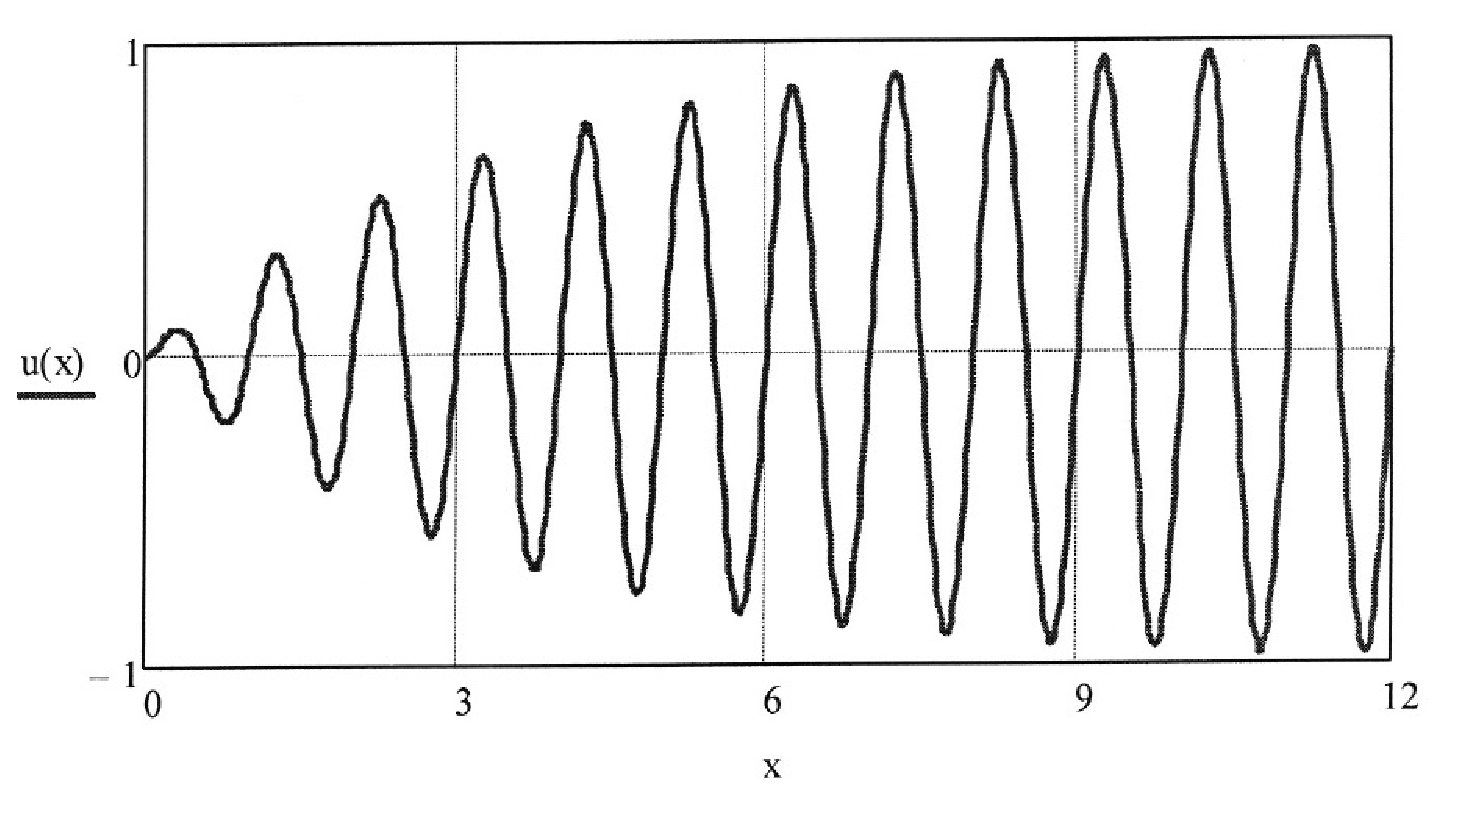
\includegraphics[width=0.6\linewidth]{Chapter_2/13}
    \caption{Волновод и примеры распределения поля} \figmark{waveguide}
\end{figure}

Для бегущих вдоль волновода волн $k_z$~---~действительная величина. Предельный
случай $k_z=0$ соответствует $k=k_x,$ что при условии $n=1$ приводит к формулам
для \important{критических длины и циклической частоты волн}, распространяющихся
в вакуумном волноводе: 
\begin{equation} 
\eqmark{2.0.2} \lambda_{\text{кр}}=2a,
\qquad \omega_{\text{кр}}=\pi c/a. 
\end{equation} 
Если $\lambda>2a$ и,
соответственно, $\omega<\pi c/a,$ то электромагнитная волна при распространении
вдоль волновода затухает.

Для бегущей волны фазовая скорость 
\begin{equation} \eqmark{2.0.3}
V_{\text{Ф}}=\omega/k_z=c/\sqrt{1-\omega^2_{\text{кр}}/\omega^2} 
\end{equation}
больше скорости света в вакууме $c,$ а длина волны в волноводе 
\begin{equation}
\eqmark{2.0.4} \lambda_{\text{В}}=\lambda_0/\sqrt{1-(\lambda_0/2a)^2}
\end{equation} больше длины волны в вакууме $\lambda_0.$ В представленном на
рис.~\figref{waveguide} случае отлична от нуля продольная составляющая
магнитного поля, и такую волну называют \important{магнитной ($H$-волна).}
Обычно для передачи СВЧ-энергии по прямоугольному волноводу используется волна
(мода) $H_{10}.$  Второй индекс $0$ соответствует отсутствию составляющей
электромагнитного поля $E_x.$ Критическая длина волны моды
$H_{10}$~---~максимальная среди всех типов волн в прямоугольном волноводе, и
поэтому ее называют \important{основной.} Тем самым, для волновода заданного
сечения существует диапазон частот, ограниченный снизу критической частотой
волны $H_{10}$ ($\lambda_{\text{кр}}=2a$). Следующая по возрастанию
частоты~---~мода $H_{01}$ с $\lambda_{\text{кр}}=2b$ или $H_{20}$ с
$\lambda_{\text{кр}}=a,$ если $a>b.$

В заданном частотном диапазоне СВЧ-энергия может переноситься одним типом волн,
что существенно облегчает её дальнейшее использование.

Если в волноводе имеется какое-либо препятствие, нерегулярность, то в нём
появляется \important{отражённая волна.} Падающая $E_0$ и отраженная волна с
коэффициентом отражения $\rho$ по амплитуде интерферируют и создают в волноводе
стоячую волну.

Максимальное (в пучности) и минимальное (в узле) значения поля равны
соответственно 
\begin{equation} \eqmark{2.0.5} 
E_{\text{max}}=E_0(1+\rho),
\qquad E_{\text{min}}=E_0(1-\rho). 
\end{equation} 
Отношение
$K=E_{\text{max}}/E_{\text{min}}$ называется \important{коэффициентом стоячей
    волны} (к.с.в.). Коэффициент отражения от препятствия по амплитуде
\begin{equation} \eqmark{2.0.6}
\rho=\dfrac{E_{\text{max}}-E_{\text{min}}}{E_{\text{max}}+E_{\text{min}}}=\dfrac{K-1}{K+1}. 
\end{equation}

В случае полного отражения (металлическая заглушка) $\rho=1,$ а если в волновод
вставлено вещество, поглощающее СВЧ-­излучение (согласованная нагрузка), то
$\rho=0.$

Для определения коэффициента стоячей волны обычно используют измерительную
линию~---~отрезок волновода с продольной щелью длиной в несколько полуволн. В
щели располагается зонд~---~большой металлический штырь (антенна), реагирующий
на электрическое поле в волноводе. Напряжение высокой частоты, наводимое на
зонд, детектируется, усиливается и подаётся на микровольтметр. Зонд может
перемещаться вдоль линии, что позволяет исследовать распределение электрического
поля в волноводе.


\introsection{Квазистационарное приближение}

Рассмотрим переменные электромагнитные поля в хорошо проводящих средах.
Если характерная частота изменения поля достаточно мала, а проводимость
среды $\lambda$, наоборот, велика, то можно пренебречь током смещения
%$\ddt{\vec{D}}\sim \omega \vec{D}$ 
по сравнению с токами проводимости $\vec{j}$.
Уравнение~\eqref{4} без тока смещения представляет собой законом Ампер 
для постоянного поля. В~дифференциальной форме:
\begin{equation}\eqmark{ampere-dif}
\Rot \vec{H} = \vec{j}.
\end{equation}
Поле и ток в среде будем считать связанными законом Ома \eqref{7} 
$\vec{j}=\lambda\vec{E}$.
При этом будем считать, что переменное магнитное поле вызывает
вихревое электрическое поле согласно закону электромагнитной индукции~\eqref{3}.
Такое приближение принято называть \term{квазистационарным}.



Выразим уравнения динамики электромагнитных полей в рассматриваемом приближении.
Подставим закон Ома в \eqref{ampere-dif} и возьмём ротор обеих частей.
С учётом соотношения \eqref{rotrot} имеем
\begin{equation*} \eqmark{8}
\nabla^2\vec{H}= -\lambda \Rot \vec{E}.
\end{equation*}
Используя уравнение электромагнитной индукции \eqref{3} с учётом материального 
уравнения \eqref{6}, получим окончательно:
\begin{equation}\eqmark{skin-H}
\nabla^2\vec{H}= \lambda\mu\mu_0 \ddt{\vec{H}}.
\end{equation}
Аналогичное уравнение имеет место и для $\vec{E}$:
возьмём ротор \eqref{skin-H} и с учётом \eqref{ampere-dif} получим
\begin{equation}\eqmark{skin-E}
\nabla^2\vec{E}= \lambda\mu\mu_0 \ddt{\vec{E}}.
\end{equation}

В отличие от случая, рассмотренного в п.~\ref{sec:emwaves}, 
полученные уравнения не являются волновыми. Математически они аналогичны
\emph{уравнению диффузии} (или \emph{уравнению теплопроводности}). Роль 
<<коэффициента диффузии поля>> играет величина
\begin{equation}
D = \frac{1}{\lambda \mu \mu_0}.
\end{equation}

\begin{lab:note}
    Уточним область применимости квазистационарного приближения.
    Пренебрежение током смещения эквивалентно предположению о бесконечной скорости 
    распространения электромагнитных волн $c\to \infty$ вне проводника. 
    На практике оно применимо, если характерные размеры системы~$l$ малы по
    сравнению с расстоянием, на которое электромагнитная волна распространится
    за характерное время $T\sim 1/\nu$ изучаемого процесса.
    Кроме того, плотность тока смещения 
    $\ddt{\vec{D}} \sim \frac{\varepsilon\varepsilon_0 \vec{E}}{T}$ 
    должна быть меньше плотности тока проводимости $\vec{j}=\lambda\vec{E}$.
    Отсюда получаем два условия на характерную частоту изменения поля:
    \[
    \nu \ll \frac{c}{l},\qquad \nu \ll \frac{\lambda}{\varepsilon\varepsilon_0}.
    \]
    Последнее условие для металлов обычно выполняется с большим запасом. 
    Например, для медного проводника $\lambda \approx 6,7\cdot 10^7$~См/м,
    имеем $\nu \ll 7\cdot 10^{18}$~Гц. Первое же ограничение является гораздо 
    более сильным: например, при характерных размерах $l\sim 1$~м необходимо
    $\nu \ll 3 \cdot 10^8$~Гц.
\end{lab:note}

%TODO: figure

%\rfr[11]{30mm}{1}{}{1}{
%\psfrag{x}[tr]{$x$}
%\psfrag{z}{$z$}
%\psfrag{a}[cl]{$E_0e^{i\omega t}$}
%\psfrag{b}[cl]{$E_x(z,\,t)$}
%}


\introsubsection{Скин-эффект}

%TODO
Рассмотрим квазистационарное поле внутри проводящей среды в простейшем --- одномерном --- случае.
Пусть вектор~$\vec{E}$ направлен всюду вдоль оси $x$ (рис.~1) и зависит 
только от координаты~$z$, т.\,е. $E_y=E_z\equiv 0$, $E_x\equiv E_x(z,\,t)$. 
Тогда уравнение \eqref{skin-E} для электрического поля будет иметь вид
\begin{equation} \eqmark{14}
\frac{\partial^2E_x}{\partial z^2}=\mu_0\mu\lambda\ddt{E_x}.
\end{equation}
Пусть полупространство $z>0$ заполнено проводящей средой с проводимостью $\lambda$, 
а на границе $z=0$ задано электрическое поле, изменяющееся по гармоническому закону: 
$E_x=E_0e^{i\omega t}$. Будем
искать решение уравнения \eqref{14} также в виде гармонической функции:
\begin{equation*} \eqmark{15}
E_x(z,\,t)=E(z)e^{i\omega t},
\end{equation*}
где $E(z)$ --- комплексная амплитуда колебаний поля, зависящая от координаты~$z$.
После подстановки в \eqref{14} получим уравнение на функцию~$E(z)$:
\begin{equation} \eqmark{16}
\frac{d^2E}{dz^2}=i\omega\cdot \lambda\mu\mu_0 E.
\end{equation}

Как известно из теории линейных дифференциальных уравнений, общее решение
\eqref{16} нужно искать в виде 
\begin{equation} \eqmark{17}
E(z)=E_0 e^{\alpha z},
\end{equation}
где $\alpha$~--- комплексная константа. 
Подставляя \eqref{17} в \eqref{16}, получим, что уравнение имеет
нетривиальные решения такого вида при
\begin{equation*} \eqmark{18}
\alpha^2=i\omega\lambda\mu\mu_0.
\end{equation*}
Отсюда
\begin{equation*}
\alpha=\pm\frac{1+i}{\sqrt{2}}\sqrt{\omega\lambda\mu\mu_0}.
\end{equation*}

Для полубесконечной среды ($z>0$) физический смысл имеет только решение
со знаком <<$-$>>, соответствующее стремлению к нулю амплитуды поля 
при $z\to \infty$. 
Окончательное решение уравнения \eqref{14} для нашего случая:
\begin{equation} \eqmark{19}
E_x(z,\,t)=E_0e^{-z/\delta}\,e^{i(\omega t- z/\delta)},
\end{equation}
где
\begin{equation} \eqmark{20}
\delta = \sqrt{\frac{2}{\omega\lambda\mu_0\mu}} = \sqrt{\frac{2D}{\omega}}.
\end{equation}
Из полученного решения \eqref{19} видно, что амплитуда переменного
электрического поля с частотой $\omega$ убывает вглубь
проводника по экспоненциальному закону. 
Такой закон спадания характеризуется расстоянием $\delta$, 
на котором амплитуда поля уменьшается в $e$ раз. 
Это расстояние называют \term{глубиной проникновения} поля
или \term{скиновой} длиной.
Как видно \eqref{20}, 
с ростом частоты $\omega$ электрическое поле всё более <<вытесняется>> 
к поверхности проводника. Это явление называется \term{скин-эффектом}. 
Поскольку уравнение для магнитного поля \eqref{skin-H} совершенно аналогично
уравнению для напряжённости электрического поля \eqref{skin-E}, то очевидно, 
что магнитное поле $H_y(z)$ убывает вглубь проводника точно по такому же закону, 
как и $E_x(z)$.

